\documentclass{article}
\usepackage{graphicx}       % For images
\usepackage{float}          % For table positioning
\usepackage[utf8]{inputenc} % UTF-8 encoding
\usepackage{listings}       % For code examples
\usepackage{xcolor}         % For coloring code (optional but helpful)

\title{Basic Python}
\author{Minh Phuoc}
\date{June 2025}

\begin{document}

\maketitle

\section{Introduction}

Data types are fundamental in programming.  
They define the kind of value a variable can hold.  
In Python, these basic data types are used to store numbers, text, and logical values.

\begin{table}[H]
\centering
\begin{tabular}{|c|l|l|}
\hline
\textbf{Data Type} & \textbf{Description} & \textbf{Examples} \\ \hline
\texttt{Integer} & Whole numbers & \texttt{1}, \texttt{-5}, \texttt{100} \\ \hline
\texttt{Float} & Decimal numbers & \texttt{3.14}, \texttt{-0.01} \\ \hline
\texttt{String} & Sequence of characters & \texttt{"Hello"}, \texttt{'Python'} \\ \hline
\texttt{Boolean} & Logical values: true or false & \texttt{True}, \texttt{False} \\ \hline
\end{tabular}
\caption{Basic data types in Python}
\end{table}

\section{List in Python}

A \textbf{list} is a collection used to store multiple items in a single variable.  
Lists can contain elements of any data type, and the items are \textbf{ordered and changeable}.

You can define a list using the following syntax:
\begin{lstlisting}[language=Python]
list_name = [element1, element2, ..., elementN]
\end{lstlisting}

For example:
\begin{lstlisting}[language=Python]
# Create a list of fruits
fruits = ["apple", "banana", "cherry"]
print(fruits[0])  # Output: apple
\end{lstlisting}

You can add, remove, or change items in a list.  
Lists are defined using square brackets \texttt{[ ]} and items are separated by commas.

\section{Dictionary in Python}

A \textbf{dictionary} is a collection of key-value pairs.  
Each item in a dictionary has a \textbf{key} and a \textbf{value}, and the key is used to access the value.  
Dictionaries are \textbf{unordered}, \textbf{changeable}, and do not allow duplicate keys.

You can define a list using the following syntax:
\begin{figure}[H]
    \centering
    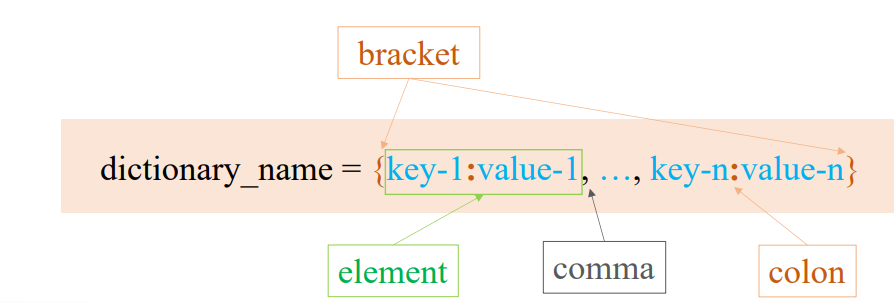
\includegraphics[width=0.75\textwidth]{dictionary_syntax.png}
    \caption{Dictionary syntax breakdown: key-value pairs inside curly brackets}
\end{figure}

Here is a simple example of a dictionary in Python:

\begin{lstlisting}[language=Python]
# Create a dictionary with student information
student = {
    "name": "Alice",
    "age": 20,
    "major": "Computer Science"
}

# Access the value using a key
print(student["name"])  # Output: Alice
\end{lstlisting}

You can update, add, or remove key-value pairs in a dictionary.  
Dictionaries are defined using curly braces \texttt{\{\}} and use colons \texttt{:} to separate keys and values.
\section{Functions in Python}

A \textbf{function} is a reusable block of code that performs a specific task.  
Functions help make your code organized, readable, and avoid repetition.

You can define a function in Python using the \texttt{def} keyword followed by the function name and parentheses.
\begin{figure}[H]
    \centering
    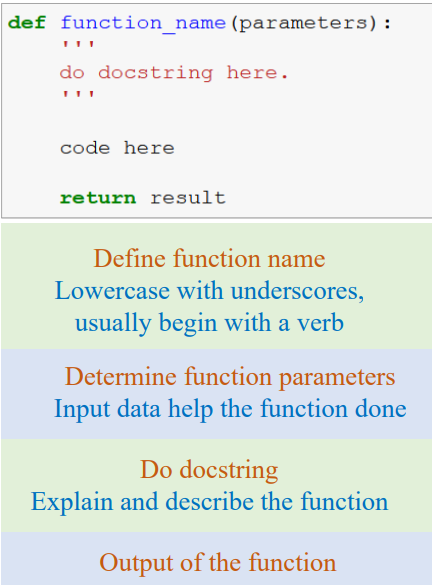
\includegraphics[width=0.7\textwidth]{function_syntax.png}
    \caption{Structure of a Python function with explanation}
\end{figure}


\begin{lstlisting}[language=Python]
# Define a simple function
def greet():
    print("Hello!")

# Call the function
greet()  # Output: Hello!
\end{lstlisting}

Functions can also take \textbf{parameters} (inputs) and return values using the \texttt{return} keyword:

\begin{lstlisting}[language=Python]
# Function with parameters and return value
def add(a, b):
    return a + b

result = add(3, 5)
print(result)  # Output: 8
\end{lstlisting}

\subsection*{Syntax Summary}
\begin{itemize}
    \item \texttt{def function\_name(parameters):} — defines a function.
    \item Indentation (usually 4 spaces) is required to define the function body.
    \item Use \texttt{return} to return a result from the function.
\end{itemize}

Functions are powerful tools to break programs into smaller, manageable parts and to reuse code efficiently.

\section{Branching in Python}

Branching allows a program to make decisions based on conditions.  
This is commonly done using \texttt{if}, \texttt{elif}, and \texttt{else} statements.

\subsection{Comparison Operators}

Comparison operators are used to compare two values.  
They return a Boolean value: \texttt{True} or \texttt{False}.  
Here are the most common comparison operators in Python:

\begin{table}[H]
\centering
\begin{tabular}{|c|l|}
\hline
\textbf{Operator} & \textbf{Description} \\ \hline
\texttt{==} & Equal to \\ \hline
\texttt{!=} & Not equal to \\ \hline
\texttt{>} & Greater than \\ \hline
\texttt{<} & Less than \\ \hline
\texttt{>=} & Greater than or equal to \\ \hline
\texttt{<=} & Less than or equal to \\ \hline
\end{tabular}
\caption{Comparison operators in Python}
\end{table}

\subsection{Using \texttt{if} Statements}

The \texttt{if} statement allows you to execute code only if a certain condition is \texttt{True}.

\begin{lstlisting}[language=Python]
age = 18
if age >= 18:
    print("You are an adult.")
\end{lstlisting}

\subsection{Using \texttt{if-else}}

You can use \texttt{else} to define an alternative block of code when the condition is not met.

\begin{lstlisting}[language=Python]
age = 16
if age >= 18:
    print("You are an adult.")
else:
    print("You are a minor.")
\end{lstlisting}

\subsection{Using \texttt{elif}}

Use \texttt{elif} (else if) to check multiple conditions.

\begin{lstlisting}[language=Python]
score = 75
if score >= 90:
    print("Grade A")
elif score >= 80:
    print("Grade B")
elif score >= 70:
    print("Grade C")
else:
    print("Grade D or lower")
\end{lstlisting}


\end{document}





